% Sources: ULXspectra docs/green_surface_monte_carlo.md; PLAN.md C18
% Code: ULXspectra, branch fix-results-integrity, commit 4da7c04 (all numbers and figures here);
%       scripts docs/scripts/mc_green_surface.py, mc_green_surface_spectra.py (added in fa567f9),
%       docs/scripts/funnel_beaming_mc.py (added in 4da7c04)
% Preliminary results (requested by the author 2026-11-01). Nothing here goes beyond the doc.

\section{Radiative transfer in the wind funnel: a Monte Carlo test}
\label{app:mc}

\subsection{What the ray cast assumes}
\label{app:mc:raycast}

The emitting surface of the wind is the surface $\taup = 1$ (Sect.~\ref{sec:wind:photosphere}), that is the last-scattering surface for photons that leave perpendicular to the disc.
In the ray cast of Sect.~\ref{sec:spectrum} every element of this surface radiates a blackbody, Lambertian about its normal, and the wind above the surface is transparent to the observer.
% source: docs/green_surface_monte_carlo.md, "What the code does"
The temperatures are normalised so that the emitted energy is right (Sect.~\ref{sec:wtemp:budget}).
The light that the surface itself blocks on the way to the observer is dropped, not redistributed, so that the energy received by observers at all inclinations, $\int L_{\rm iso}\,{\rm d}\mu$, is below the emitted energy.
For the three fits of this appendix the share of the emitted energy that reaches observers is 0.86 (\srcHoIX), 0.95 (\srcNGCthirteen) and 0.50 (\srcNGCfiftyfour).
% source: docs/green_surface_monte_carlo.md, table "share of emitted energy that reaches observers"; commit 4da7c04
% Source names: macros in main.tex (author 2026-11-01: full names; NGC1313B to be decided)

Seen obliquely, the surface of the last scattering lies elsewhere.
In a plane-parallel scattering atmosphere the surface $\tau = 1$ along a ray at the cosine $\mu$ to the normal lies at $\taup = \mu$, slightly above the surface $\taup = 1$.
This is limb darkening: for pure electron scattering \citep{Chandrasekhar1960}
\begin{equation}
\frac{I(\mu)}{I_{\rm Lambert}} = \frac{1 + 2.06\,\mu}{2.373} ,
\label{eq:mc_limb}
\end{equation}
% source: docs/green_surface_monte_carlo.md, "Analytic expectations" (Chandrasekhar)
which is 1.29 at $\mu = 1$, 0.86 at $\mu = 0.5$ and 0.42 at $\mu \to 0$.
The Lambertian elements of the code give the same total, but miss this redistribution over angles by 30--60 per cent.
In an extended wind with $\rho \propto r^{-2}$ the optical depth from the distance $r$ to infinity along a straight ray at the angle $\psi$ to the radius vector is $\tau = \tau_r\,\psi/\sin\psi$, where $\tau_r = \kT\rho r$ is the radial optical depth.
% derived (Claude, 2026-11-01): impact parameter b = r sin(psi); int_{r cos psi}^inf ds/(b^2 + s^2) = psi/b,
%         so tau = kappa rho r^2 psi/b = tau_r psi/sin(psi)
Since $\tau_r \propto 1/r$, the photosphere seen along rays leaving at $\psi$ lies at $\psi/\sin\psi$ times the radius of the radial one, that is further out by at most a factor $\pi/2$ for the rays that point outwards, $\psi \le \pi/2$.
% source: docs/green_surface_monte_carlo.md, "Analytic expectations" (factor psi/sin psi <= pi/2); psi defined by Claude (author 2026-11-01: define)
Neither estimate covers the case that dominates in our fits.
Where $\taup < 1$ through the whole wind, the surface $\taup = 1$ lies on the disc, yet an inclined ray crosses the wind cone over a long path, and the optical depth along it is $\gg 1$.

\subsection{Method}
\label{app:mc:method}

We followed photon packets with a Monte Carlo code (\code{docs/scripts/mc\_green\_surface.py} in the code repository).
The packets start on the emitting surface of the model, with the temperatures of the model: the wind photosphere and the directly seen disc inside $\rout$.
They are drawn in proportion to $T^4\,{\rm d}A$ and emitted Lambertian about the local normal, as in the ray cast.
% source: docs/green_surface_monte_carlo.md, "Monte Carlo"; mc_green_surface.py docstring
We considered two cases, which differ only in what happens to a packet after it leaves the surface.
\begin{itemize}
\item \emph{Scattering:} the packets scatter on electrons in the wind density of the model (Sect.~\ref{sec:wind:density}, with the ballistic speed law) until they escape.
Scattering is Thomson, isotropic and conservative, without change of photon energy, and the disc plane reflects diffusely with the albedo of unity.
This is the physical case within these assumptions.
\item \emph{Reflection:} the wind has no opacity, and the surface $\taup = 1$ is an opaque diffuse mirror.
This is the geometry of the ray cast, but with the blocked light kept.
\end{itemize}
% source: docs/green_surface_monte_carlo.md, "Monte Carlo" and the table "How to read the lines"
The ratio of the reflection case to the ray cast thus gives the effect of dropping the occulted light.
The ratio of the scattering case to the reflection case gives the effect of the wind above the surface $\taup = 1$, that is of defining the emitting surface by $\taup$.
The ray cast of the code is reproduced in the script; at the best-fit inclination it gives the bolometric $L_{\rm iso}$ within 1.5 per cent of the code.
% source: docs/green_surface_monte_carlo.md, "Monte Carlo" (Lbol_iso within 1.5% of model_energy_report.txt)

We used the best fits of \srcHoIX, \srcNGCthirteen and \srcNGCfiftyfour with the preset BH3a over the full energy range, with $4\times10^4$ packets per run (Table~\ref{tab:mc_fits}).
All three have $\theta_{\rm c} = 45.6^\circ$ ($\omf = 0.7$) and $\theta_{\rm d} = 90^\circ$, so that the edge of the funnel is at $i \approx 46^\circ$.
% source: docs/green_surface_monte_carlo.md, "Monte Carlo" (fits, packets, theta_c, theta_d)
The preset BH3a is the main model (Sect.~\ref{sec:model}) for a BH with $\Rsph$ from the condition~\eqref{eq:rsph_Ledd}.
Its free parameters are $M$, $\mdot_0$, $f_{\rm in}$, $r_{\rm in,f}$, $\rout$, $i$, $\epsilon_{\rm w}$ and $\beta_{\rm w}$; $\omf = 0.7$ and $\hd = 0$ are fixed (Table~\ref{tab:params}).
The full energy range means all the points of the observed SED.
% code: ULX.conf [BH3a] (wind_scenario = set_mdot_in, use_simple_rsp = 2, free_params, dip = 0) and [DEFAULT]
%       (omega_frac = 0.7, h_disc = 0); run tag "full": run_adaptive_fits.sh ... full "BH2 BH3a" --Emax 1e3 (README)
% AUTHOR: check that the Ledd rule is use_simple_rsp = 2 (Sect. radii) and the meaning of "full".

\begin{table}
\centering
\caption{Best fits used in the Monte Carlo test (preset BH3a, full energy range): inclination, share of the wind in the emitted luminosity $L_{\rm w}/L$, number of scatterings per packet (median and 90th percentile) and share of packets that escape without scattering (unscatt.).}
\label{tab:mc_fits}
\small
\setlength{\tabcolsep}{4pt}
\begin{tabular}{@{}lcccc@{}}
\toprule
Source & $i_{\rm best}$ & $L_{\rm w}/L$ & scatterings & unscatt. \\
\midrule
\srcHoIX & $9.2^\circ$ & 0.011 & 3, 24 & 30\% \\
\srcNGCthirteen & $19.5^\circ$ & 0.001 & 2, 16 & 32\% \\
\srcNGCfiftyfour & $48.5^\circ$ & 0.93 & 32, 1207 & 11\% \\
\bottomrule
\end{tabular}
% source: docs/green_surface_monte_carlo.md, table after "Fits:"; commit 4da7c04
\end{table}

\subsection{Spectra and luminosity against inclination}
\label{app:mc:spectra}

Figure~\ref{fig:mc_spectra} compares the intrinsic spectra, without absorption, of the ray cast and of the two Monte Carlo cases, and Table~\ref{tab:mc_ratio} gives the bolometric ratios.
The result depends on whether the line of sight lies inside the funnel, $i < \theta_{\rm c}$, or crosses the wind cone, $i > \theta_{\rm c}$.

Inside the funnel the ray cast underestimates $L_{\rm iso}$ by a factor of 1.5--2.4, and the shape of the spectrum above about 0.1~keV hardly changes.
For \srcHoIX at $9^\circ$ and \srcNGCthirteen at $19^\circ$ the ratio is flat to within about 10 per cent from 0.3 to 30~keV.
The factor has two parts.
The occulted light that the ray cast drops contributes a factor of 1.05--1.15 for \srcHoIX and \srcNGCthirteen and of 2.0 for the wind-dominated \srcNGCfiftyfour.
The rest, a factor of 1.2--1.8, is the collimation by the funnel: light scattered off the funnel walls leaves along the axis (Sect.~\ref{app:mc:funnel}).
% source: docs/green_surface_monte_carlo.md, "Conclusions" item 2; commit 4da7c04

Beyond the edge of the funnel the error is large.
The line of sight crosses the wind cone, which is thin perpendicularly but thick obliquely.
The ray cast treats the wind above the surface $\taup = 1$ as transparent and still sees the hot inner disc.
For \srcHoIX and \srcNGCthirteen it overestimates $L_{\rm iso}$ by a factor of 2.5--8 at $50$--$63^\circ$ (\srcNGCthirteen up to $75^\circ$), and its spectrum is too hard: the ratio of the Monte Carlo to the ray cast falls from 0.3--0.7 below 0.1~keV to 0.1--0.3 at 10~keV.
Close to the disc plane the ray cast gives no hard flux at all, while the scattered light keeps a hard tail.
The ratios above unity at the largest inclinations in Table~\ref{tab:mc_ratio} (\srcHoIX at $70^\circ$, \srcNGCfiftyfour at $63$--$70^\circ$) do not mean that the Monte Carlo is bright there.
They arise because the ray cast becomes dark: the outer part of the emitting surface hides the inner disc from the observer.
In \srcHoIX the wind photosphere rises to $z/R = 0.39$ at $x \approx 490$, which hides the surface well inside this radius for $i \gtrsim 68.5^\circ$, and $L_{\rm iso}/L_{\rm total}$ of the ray cast drops from 0.90 at $63^\circ$ to 0.033 at $70^\circ$.
In \srcNGCfiftyfour the photosphere reaches $z/R = 0.88$ at $x \approx 320$, so the hiding begins at $i \approx 49^\circ$, and $L_{\rm iso}/L_{\rm total}$ of the ray cast falls from 0.19 at $57^\circ$ to 0.015 at $70^\circ$.
The Monte Carlo, in contrast, changes smoothly with $i$: the light that leaks out of the funnel through the wind gives $L_{\rm iso}/L_{\rm total} \approx 0.06$--$0.09$ in both cases, and the reflection case keeps the light that the surface blocks.
In \srcNGCthirteen the photosphere is lower, $z/R \le 0.24$, the hiding begins only at $i \approx 77^\circ$, and the ratio stays below unity up to $75^\circ$.
% derived (Claude, 2026-11-01) at the request of the author ("explain"): max z_ph/x of
%   results/mcmc_{HolmIX,NGC1313B,NGC5408}.BH3a.full/surface_Python.dat (0.394 at x = 489; 0.237 at x = 647;
%   0.882 at x = 320), i = 90 deg - arctan(max z/x); code and MC L_iso/L_tot per bin from mc_results.txt of the
%   MC runs of 2026-10-31 (mc_green_surface.py, the runs behind docs/green_surface_monte_carlo.md, commit 4da7c04):
%   HolmIX code 0.899 (63.3), 0.033 (69.5); MC scatter 0.105, 0.087; NGC5408 code 0.185 (56.6), 0.053, 0.015 (69.5);
%   MC scatter 0.130, 0.075, 0.061. Not in the doc.
% source: docs/green_surface_monte_carlo.md, "Conclusions" item 1; commit 4da7c04
The surface $\taup = 1$ is therefore a good emitting surface for oblique views only where the wind is optically thick perpendicularly.
Where it is thin perpendicularly, which is most of the surface in \srcHoIX and \srcNGCthirteen, the surface seen obliquely is a different one, the wind cone itself.
% source: docs/green_surface_monte_carlo.md, "Conclusions" item 3

The best-fit inclination of \srcNGCfiftyfour, $48.5^\circ$, lies just beyond the edge of the funnel, where both the ray cast and the Monte Carlo change fastest with $i$.
In the bin $45$--$52^\circ$ the bolometric ratio is 0.91, because the dropped light and the hidden centre nearly cancel, and the spectrum above 3~keV is about 30 per cent softer in the Monte Carlo.
This agreement is a coincidence, and the posterior of $i$ near the edge of the funnel is not reliable.
% source: docs/green_surface_monte_carlo.md, "Conclusions" item 5

The total emitted energy does not depend on the choice of the emitting surface, because it is fixed by $f_{\rm cor}$ (Eq.~\ref{eq:fcor}), and the temperatures depend on it only weakly, $T \propto A^{-1/4}$, by at most 25 per cent.
What an observer at a given $i$ receives depends on this choice strongly, through the projected area, the occultation and the dropped light.
The fitted parameters absorb this error.
% source: docs/green_surface_monte_carlo.md, "Conclusions" item 4

\begin{table*}
\centering
\caption{Bolometric $L_{\rm iso}(i)$ of the Monte Carlo divided by that of the ray cast, for the scattering and the reflection cases, in bins $\Delta\mu = 0.1$. At $i \ge 76^\circ$ the ray cast gives $L_{\rm iso} \approx 0$ (for \srcNGCthirteen beyond the first bin, where the scattering ratio is 0.18).}
\label{tab:mc_ratio}
\small
\begin{tabular}{@{}lcccccc@{}}
\toprule
& \multicolumn{2}{c}{\srcHoIX} & \multicolumn{2}{c}{\srcNGCthirteen} & \multicolumn{2}{c}{\srcNGCfiftyfour} \\
$i$ & scattering & reflection & scattering & reflection & scattering & reflection \\
\midrule
$18^\circ$ & 1.95 & 1.15 & 1.85 & 1.05 & 2.35 & 1.99 \\
$32^\circ$ & 1.80 & 1.14 & 1.72 & 1.05 & 2.29 & 1.98 \\
$41^\circ$ & 1.58 & 1.16 & 1.55 & 1.07 & 2.24 & 1.97 \\
$50^\circ$ & 0.27 & 1.16 & 0.40 & 1.07 & 0.70 & 2.13 \\
$57^\circ$ & 0.14 & 1.13 & 0.20 & 1.04 & 0.70 & 2.54 \\
$63^\circ$ & 0.12 & 1.14 & 0.18 & 1.06 & 1.42 & 2.63 \\
$70^\circ$ & 2.6 & 10 & 0.16 & 1.05 & 4.0 & 2.8 \\
\bottomrule
\end{tabular}
% source: docs/green_surface_monte_carlo.md, "Results" table; commit 4da7c04
\end{table*}

\begin{figure*}
\centering
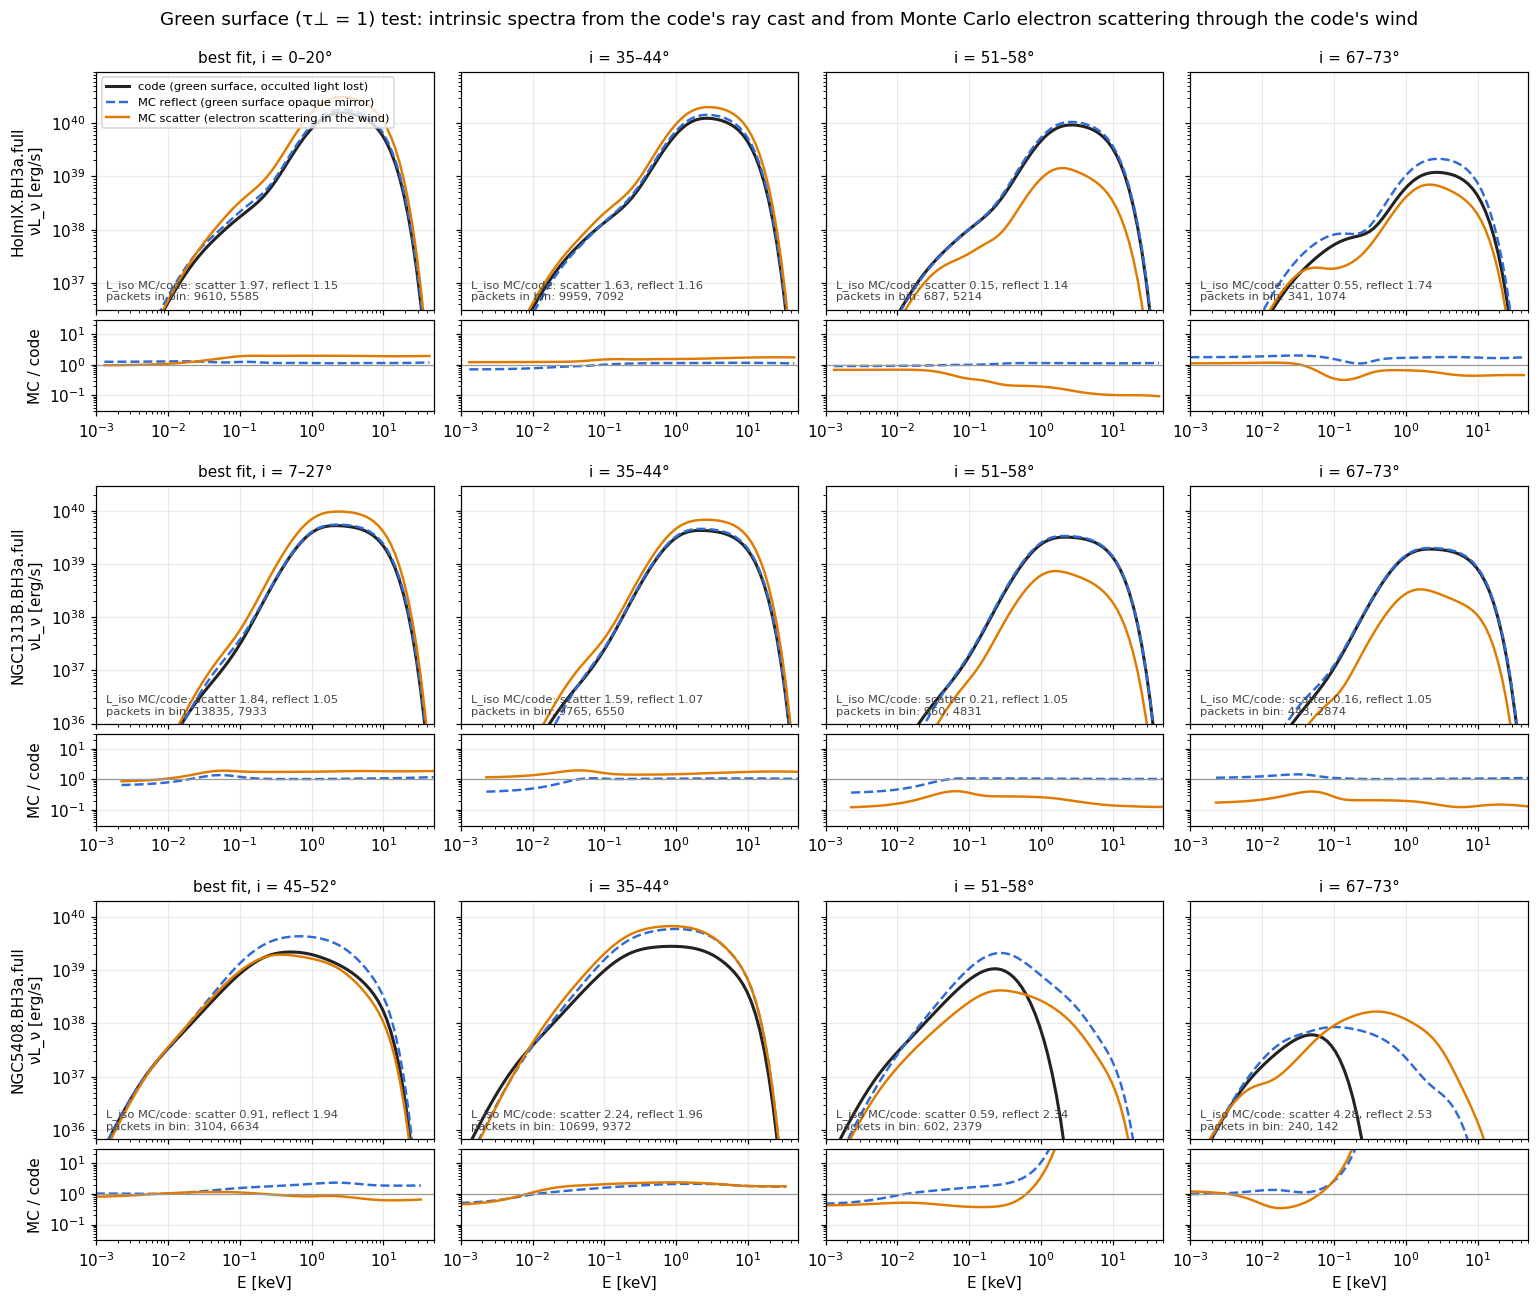
\includegraphics[width=\textwidth]{mc_green_surface_spectra.png}
\caption{Intrinsic spectra $\nu L_\nu$ (no absorption) of the best fits of \srcHoIX, \srcNGCthirteen and \srcNGCfiftyfour (rows; preset BH3a, full energy range) in bins $\mu \pm 0.05$ around the best-fit inclination, $40^\circ$, $55^\circ$ and $70^\circ$ (columns).
Black: the ray cast of the code (surface $\taup = 1$, occulted light lost).
Blue dashed: Monte Carlo with the surface $\taup = 1$ as an opaque diffuse mirror.
Orange: Monte Carlo with electron scattering in the wind of the model.
The lower panels show the ratio of the Monte Carlo to the ray cast.
Made with \code{docs/scripts/mc\_green\_surface.py} and \code{mc\_green\_surface\_spectra.py} (code commit fa567f9).}
\label{fig:mc_spectra}
% figure: ULXspectra docs/figures/mc_green_surface_spectra.png, commit fa567f9 (unchanged at 4da7c04)
\end{figure*}

\subsection{Collimation by the funnel: comparison with Ahlberg et al.}
\label{app:mc:funnel}

\citet{Ahlberg2026} computed the geometric beaming by a funnel in the shape of a conical frustum with infinitely optically thick, conservative walls and a point source at the centre of its base.
Their walls re-emit as Lambertian surfaces or reflect as an electron-scattering atmosphere; the two differ in the boost by at most 6 per cent.
% source: docs/green_surface_monte_carlo.md, "Funnel collimation from Ahlberg et al. (2026)", "Their model"
They define the boost of the apparent luminosity $B(i)$ by $L_{\rm app}(i) = B(i) \int F\,{\rm d}\Omega$.
Averaged over $i \le \alpha$, where $\alpha$ is the half-opening angle of the funnel, its geometric limit is (their Eq.~7)
\begin{equation}
B_{\rm max} = \frac{1}{1 - \cos\alpha} ,
\label{eq:mc_Bmax}
\end{equation}
% source: Ahlberg et al. 2026, Eq. 7, as quoted in docs/green_surface_monte_carlo.md
and the mean boost inside the funnel is approximated to about 10 per cent by (their Eq.~15)
\begin{equation}
\frac{\ln B}{\ln B_{\rm max}} \approx \exp\left(1.14\,\frac{\ln\sin\alpha}{\ln R}\right) ,
\label{eq:mc_AhlbergB}
\end{equation}
% source: Ahlberg et al. 2026, Eq. 15, as quoted in docs/green_surface_monte_carlo.md
where $R$ is the distance from the centre of the base to the edge of the funnel in units of the base radius.
% VERIFY: Eqs. (mc_Bmax), (mc_AhlbergB) against arXiv:2610.23089
In our wind, the innermost streamline is a straight cone at $\theta_{\rm c}$ from the axis starting at $\rin$, which is their geometry with $\alpha = \theta_{\rm c} = 45.6^\circ$.
% source: docs/green_surface_monte_carlo.md, "Comparison with our MC"

We first reproduced their setup with a Monte Carlo of our own (\code{docs/scripts/funnel\_beaming\_mc.py}): a conical frustum with Lambertian walls, an isotropic point source, and the plane $z = 0$ as a mirror for the lower half of the funnel, $4\times10^4$ packets per point.
% source: funnel_beaming_mc.py docstring and cone_mc(alpha, R, n=40000) for the validation; commit 4da7c04
The mean boost in the funnel agrees with their Eq.~\eqref{eq:mc_AhlbergB} within 1--13 per cent (Fig.~\ref{fig:funnel_validation}); Eq.~\eqref{eq:mc_AhlbergB} lies above our points at small $R$ and below them at large $R$, as \citet{Ahlberg2026} note.
Against their Fig.~4b, read by eye, we obtain $B/B_{\rm max} = 0.90$ at $R = 10^2$ and 0.96 at $R = 10^3$ for $\alpha = 45^\circ$ (theirs: 90 per cent at $R \approx 2\times10^2$, 95 per cent at $R \approx 1.5\times10^3$), 0.73 for $\alpha = 25^\circ$ and $R = 10^3$ (theirs about 72 per cent), and 0.31 for $\alpha = 10^\circ$ and $R = 10^3$ (theirs about 33 per cent).
For the narrow and long funnel $\alpha = 10^\circ$, $R = 10^5$, our 0.50 (Eq.~\ref{eq:mc_AhlbergB}: 0.51) is about 20 per cent above the 0.40--0.42 of their figure and text; we have no explanation, but the difference is irrelevant for $\alpha \approx 46^\circ$.
% source: docs/green_surface_monte_carlo.md, "Our opaque-cone MC vs Ahlberg et al."; commit 4da7c04

\begin{figure}
\centering
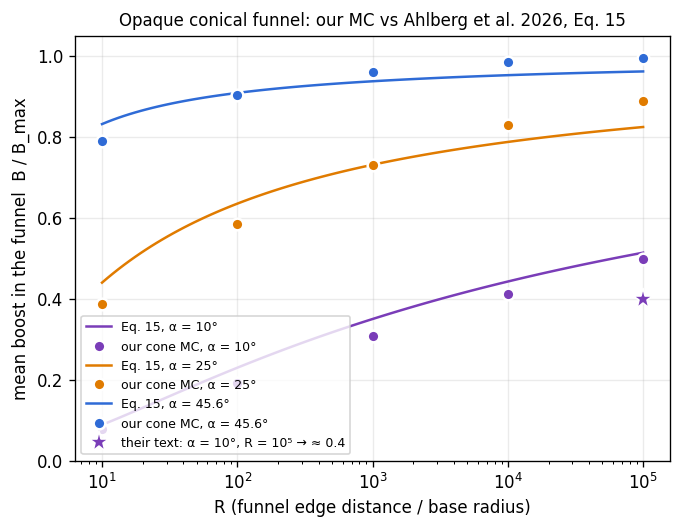
\includegraphics[width=\columnwidth]{funnel_beaming_validation.png}
\caption{Mean boost inside an opaque conical funnel, $B/B_{\rm max}$, against the distance $R$ of the funnel edge in units of the base radius, for $\alpha = 10^\circ$, $25^\circ$ and $45.6^\circ$.
Lines: Eq.~\eqref{eq:mc_AhlbergB} \citep[Eq.~15 of][]{Ahlberg2026}; dots: our Monte Carlo in their setup; star: the value quoted by \citet{Ahlberg2026} for $\alpha = 10^\circ$, $R = 10^5$.
Made with \code{docs/scripts/funnel\_beaming\_mc.py} (code commit 4da7c04).}
\label{fig:funnel_validation}
% figure: ULXspectra docs/figures/funnel_beaming_validation.png, commit 4da7c04
\end{figure}

The scattering case of Sect.~\ref{app:mc:method} agrees with the opaque cone in the mean (Table~\ref{tab:mc_funnel}).
For $\alpha = 45.6^\circ$ and $R = 10^2$--$10^4$, Eq.~\eqref{eq:mc_AhlbergB} gives $B = 3.02$--$3.17$ ($B_{\rm max} = 3.33$), and our wind gives 2.92--3.05, with 88--92 per cent of the light escaping inside the funnel.
The agreement is about 5 per cent, although the walls of our funnel are semi-transparent (2--32 scatterings in the median, Table~\ref{tab:mc_fits}) and our source is extended, the disc under the wind or the wind photosphere, rather than a point.
% source: docs/green_surface_monte_carlo.md, "Comparison with our MC" table and paragraph; commit 4da7c04

\begin{table}
\centering
\caption{Collimation by the funnel, $\alpha = \theta_{\rm c} = 45.6^\circ$: share of the light escaping at $i < \theta_{\rm c}$ and the mean boost $B$ there.}
\label{tab:mc_funnel}
\small
\begin{tabular}{@{}lcc@{}}
\toprule
& share at $i < \theta_{\rm c}$ & $B$ \\
\midrule
Eq.~\eqref{eq:mc_AhlbergB}, $R = 10^2$--$10^4$ & 1 & 3.02--3.17 \\
\srcHoIX, scattering & 0.91 & 3.04 \\
\srcNGCthirteen, scattering & 0.88 & 2.92 \\
\srcNGCfiftyfour, scattering & 0.92 & 3.05 \\
reflection (all three) & 0.54--0.79 & 1.8--2.6 \\
\bottomrule
\end{tabular}
% source: docs/green_surface_monte_carlo.md, "Comparison with our MC (scatter mode, 2026-10-31)"; commit 4da7c04
\end{table}

The angular distributions differ more than the means (Fig.~\ref{fig:funnel_wind}).
Inside the funnel, $B(i) = L_{\rm iso}(i)/L_{\rm total}$ of the wind is steeper than that of the opaque cone: 3.6--3.8 near the axis (cone 3.3--3.5) and 2.2--2.5 just inside the edge (cone 2.9).
Beyond $\theta_{\rm c}$ the wind leaks light with $B \approx 0.1$--$0.7$, and the opaque cone almost none.
% source: docs/green_surface_monte_carlo.md, "B(i) cone vs wind"; commit 4da7c04
The light emitted at different radii is collimated alike: inside the funnel its $B(i)$ is the same within about 10 per cent (Fig.~\ref{fig:funnel_radius}).
Only the outermost wind photosphere of \srcNGCfiftyfour ($x > 300$, 25 per cent of the luminosity) gives a flatter $B(i)$ and leaks more.
% source: docs/green_surface_monte_carlo.md, "B(i) by emission radius"; commit 4da7c04
For this reason the share of the luminosity above 1~keV in the Monte Carlo is constant within 1--2 per cent inside the funnel.
In the ray cast it is constant as well, because the directly seen surface is nearly flat and all rings scale as $\cos i$.
Beyond $\theta_{\rm c}$ the Monte Carlo spectrum is softer than inside, because the hot centre is hidden.
% source: docs/green_surface_monte_carlo.md, "Spectral shape against i"; commit 4da7c04

\begin{figure}
\centering
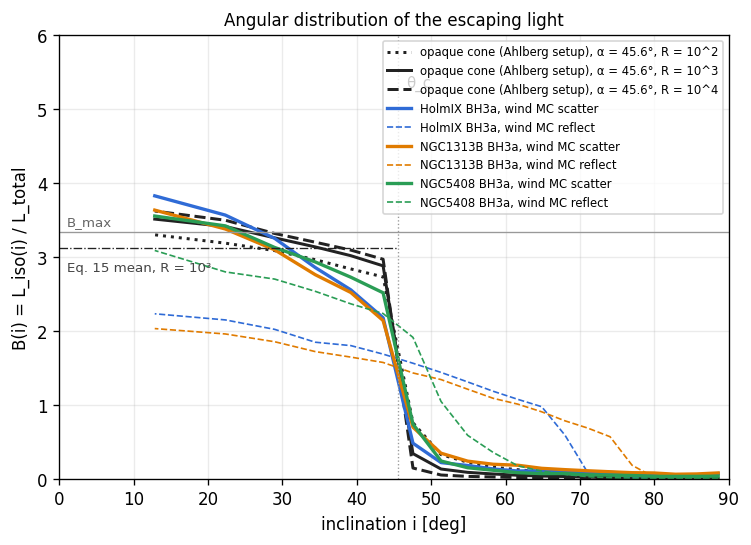
\includegraphics[width=\columnwidth]{funnel_beaming_vs_wind.png}
\caption{Angular distribution of the escaping light, $B(i) = L_{\rm iso}(i)/L_{\rm total}$, in 20 bins in $\mu$.
Black: opaque cone in the setup of \citet{Ahlberg2026}, $\alpha = 45.6^\circ$, $R = 10^2$, $10^3$, $10^4$.
Colours: Monte Carlo through the wind of the three best fits, scattering (solid) and reflection (dashed).
Made with \code{docs/scripts/funnel\_beaming\_mc.py} (code commit 4da7c04).}
\label{fig:funnel_wind}
% figure: ULXspectra docs/figures/funnel_beaming_vs_wind.png, commit 4da7c04
\end{figure}

\begin{figure*}
\centering
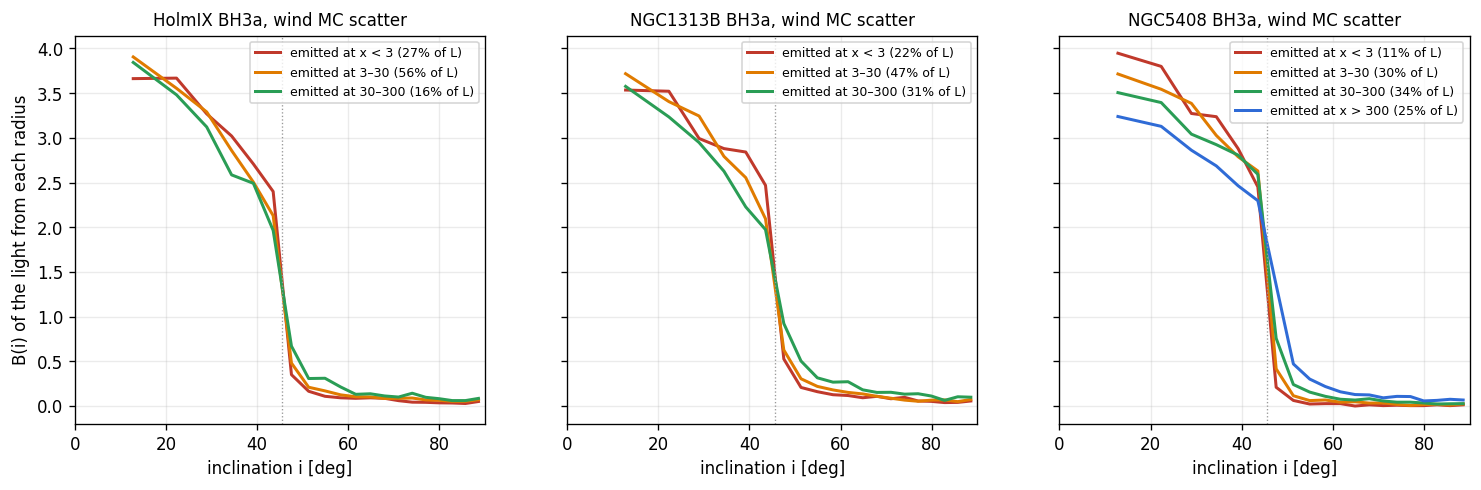
\includegraphics[width=\textwidth]{funnel_beaming_by_radius.png}
\caption{$B(i)$ of the light emitted at different radii $x = R/\rin$, Monte Carlo with scattering through the wind of the three best fits; the share of the luminosity emitted in each range is given in the legends.
The dotted line marks $\theta_{\rm c}$.
Made with \code{docs/scripts/funnel\_beaming\_mc.py} (code commit 4da7c04).}
\label{fig:funnel_radius}
% figure: ULXspectra docs/figures/funnel_beaming_by_radius.png, commit 4da7c04
\end{figure*}

\subsection{Limits of the test}
\label{app:mc:limits}

These results are preliminary.
The scattering is grey: isotropic Thomson scattering, without the Rayleigh phase function, without Doppler shifts or bulk Comptonization by the outflow, and without thermal Comptonization.
There is no absorption: a packet keeps the energy of the element that emitted it, and there is no thermalisation below the surface.
The disc plane has the albedo of unity.
The packets start on the surfaces of the model, so the test covers the transfer after emission, not where the light is emitted.
With $4\times10^4$ packets per run, a few hundred packets fall into each bin at $i \ge 70^\circ$.
% source: docs/green_surface_monte_carlo.md, "Limits of the Monte Carlo"
Only the BH fits were tested.
For a NS the Monte Carlo needs the disc surface ($\hd > 0$) and the magnetosphere as emitters and reflectors, the base of the funnel at the inner launch radius of the wind, and, for the central emitter up to about 30~keV, energy change in scattering.
% source: docs/green_surface_monte_carlo.md, "Limits" (BH fits only) and "NS fits"

% OUTLINE: what follows for the fits is the author's decision (docs/green_surface_monte_carlo.md,
%          "Possible next steps"; PLAN.md C18): inclination prior i < theta_c; energy conservation
%          in the ray cast; attenuation exp(-tau_los) along the line of sight; MC-calibrated
%          angular redistribution b(i; alpha, R) from the opaque cone + f_leak from the wind MC.
% AUTHOR: state here which of these (if any) the paper adopts, or move to the Discussion.
